\chapter{Introduction}
\label{Introduction}
\graphicspath{{Figures/Introduction/}{Figures/Common/}}

It is hard to underestimate the effect that the laser has had since its invention in 1960 \citep{Maiman:1960}.  Although initially motivated by pure scientific curiosity, its unique properties have given it application in an astonishing array of technologies, in addition to its use as a powerful tool in fundamental research.  

Laser radiation is distinguished from the light emitted by everyday light sources --- such as light bulbs --- by three main properties, (i) its narrow divergence, (ii) the narrow range of frequencies that are emitted, and (iii) the \emph{coherence} of the emitted radiation.  Although many applications only make use of the first two properties, the coherence of a laser is critical to its use in such applications as laser gyroscopes, gravitational wave detection and fundamental tests of quantum mechanics\footnote{FIXME: Add citations}.  Crudely, the coherence of light is related to the extent to which knowledge of its phase at one instant can be used to predict its phase at later times.  Light emitted from a light bulb is chaotic: its phase evolves randomly in time.  Light emitted from a laser is highly predictable: its phase evolves linearly in time with some phase diffusion over longer time scales.  

Quantum mechanics tells us that not only can light behave as a wave, but atoms can too.  This wave nature of atoms is usually indiscernible because the typical wavelength for a thermal atom is many orders of magnitude smaller than the inter-atomic spacing ($\lambda \sim 5 \times\unit[10^{-11}]{m}$ as compared to $d \sim 3 \times\unit[10^{-9}]{m}$).  However, in 1925 Einstein predicted \citep{Einstein:1925} that if a gas of \emph{bosons} (a class of particles which includes many atomic species) was cooled below a critical temperature, a large fraction of the particles would occupy the ground state of the system, forming a coherent wavefunction.  This was achieved in 1995 for dilute atomic gases \citep{Anderson:1995vn,Bradley:1995ys,Davis:1995} with the first production of a Bose-Einstein Condensate (BEC), a macroscopic occupation of atoms in a single spatial mode.  As it is the macroscopic occupation of \emph{photons} in a single spatial mode that gives the optical laser many of its properties, with the achievement of BEC it has become possible to consider the creation of an atomic analogue of the optical laser: the \emph{atom} laser.

An atom laser, while ideally sharing the above properties of its optical cousin, would behave very differently to an optical laser.  While photons interact strongly with matter, they interact only weakly with themselves or with gravity.  While this makes lasers robust to fluctuations in electromagnetic or gravitational fields, they are therefore less sensitive to these fields in interferometry experiments.  Despite this limitation, optical interferometry has been used in several incredible gravitational experiments, including GRACE, LIGO, and Gravity Probe-A \citep{Vessot:1980}.

Somewhere the award of the Nobel prizes for BEC and related work should be mentioned as it is a rapidly evolving, and exciting field of tremendous importance.  Or something.


it means that they are less sensitive to these effects in interferometry experiments where they are under investigation.  


amazing gravity experiments with lasers: GRACE, LIGO, eventually, LISA

they do not interact strongly with themselves or with gravity.  

It is the narrow spectral linewidth, the high spectral intensity, and its large coherence length that give the optical laser such a wide range of applications.  These properties themselves derive from the macroscopic occupation of photons in a single optical mode inside the laser cavity.  With the achievement of Bose-Einstein Condensate (BEC) in 1995 \citep{Anderson:1995vn,Bradley:1995ys,Davis:1995} --- a macroscopic occupation of \emph{atoms} in a single spatial mode --- there has arisen the experimental challenge of producing an atomic analogue of the optical laser: the \emph{atom} laser.  As atoms interact more readily with their environment than photons, atom interferometry has a broad range of applications: to the measurement of electric and magnetic fields in tests of atom and neutron charge neutrality \citep{Arvanitaki:2007}, an application which would be essentially impossible with optical lasers due to the weak photon--photon interaction; to fundamental tests of predictions of General Relativity \citep{Dimopoulos:2007uq}; to the development of gyroscopes \citep{Gustavson:1997}, gradiometers \citep{Snadden:1998,McGuirk:2002} and gravimeters \citep{Peters:2001}, which, while possible using optical lasers, their atomic counterparts are far more compact due to the significantly stronger gravitational interaction.

more broadly and to the development of more compact sensors.  




Although the low kinetic energy of atom lasers would prevent their use 


The differences between an atom laser and an optical laser derive from the inherent differences between photons and atoms: atoms interact much more readily with their environment.  This is both a blessing and a curse.  It is a blessing

 over an optical laser derives from the 



First cw optical laser \citep{Javan:1961}.


The achievement of Bose-Einstein Condensate (BEC) in 1995 \citep{Anderson:1995vn,Bradley:1995ys,Davis:1995} has led to the possibility of creating an analogous source for atoms, which could take advantage of the inherent differences between photons and atoms.  Atoms interact much more readily with their environment, giving atom interferometry applications in fundamental tests of predictions of General Relativity \citep{Dimopoulos:2007uq}, tests of atom and neutron charge neutrality \citep{Arvanitaki:2007}, gyroscopes \citep{Gustavson:1997}, gradiometers \citep{Snadden:1998,McGuirk:2002} and gravimeters \citep{Peters:2001}.  FIXME: How many of these actually use atom lasers, and how many use thermal beams?

The increased interactivity of atoms over photons is both a blessing and a curse: while it is the source of crap.

far more sensitive to fluctuations in external electric or magnetic fields, etc


We need to talk about thermal beams, briefly.

Discussion of cold thermal atom interferometry, and how this can be improved through the use of atom lasers. 

Rotation sensing using cold thermal atom clouds: \citep{Canuel:2006}, measuring Newton's constant $G$: \citep{Lamporesi:2008}


Here goes the motivation.

Steal everything that we can from papers.

\section{Lasers and Atom lasers}

The basic features necessary of a continuous atom laser are analogous to the features of a continuous optical laser: a resonant, a lasing mode, an outcoupling process, and a Bose-stimulated pumping mechanism (see \figureref{Introduction:LaserAtomLaserComparison}).  The first three of these features are well understood for an atom laser; experimentally realising the fourth, the pumping mechanism, has presented the greatest challenge.

\begin{figure}
    \centering
    \includegraphics[width=14cm]{LaserAtomLaserComparison}
    \caption{
        \label{Introduction:LaserAtomLaserComparison}
        FIXME: This is not a caption.
    }
\end{figure}

\subsection{The resonator}

In an optical laser, the resonator is typically a cavity formed between two (or more) mirrors trapping the photons with a region of space; the optical mode trapped within the resonator is the lasing mode.  For atom laser, the resonator is an `atom trap', either an optical trap using the ac Stark shift to trap the atoms in a region of high optical intensity, or a magnetic trap using the Zeeman shift to selectively trap certain magnetic hyperfine states near a local minimum of the magnetic field.

\subsection{The lasing mode}

\begin{figure}
    \centering
    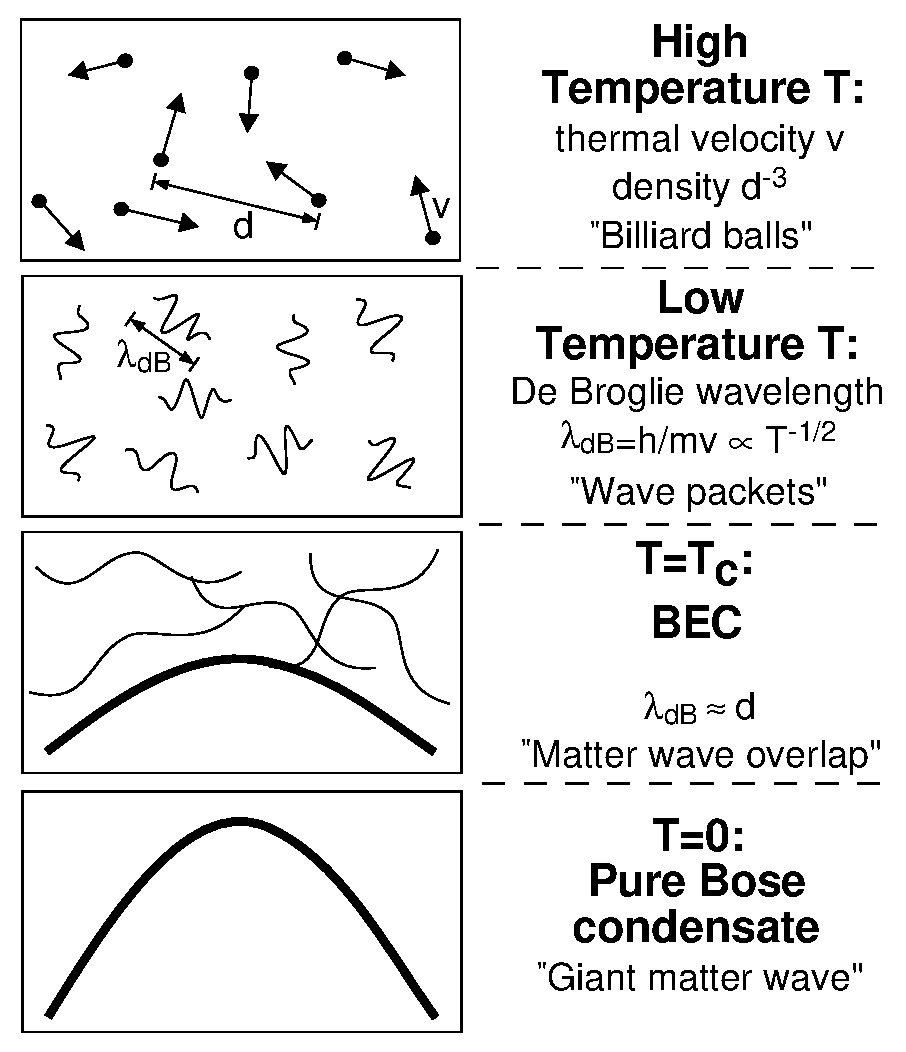
\includegraphics[width=8cm]{WhatIsBEC}
    \caption{
        \label{Introduction:WhatIsBEC}
        FIXME: This is not a caption.  Figure stolen without permission from \citep{Ketterle:1999fk}.
    }
\end{figure}

The necessary property for the lasing mode of a laser --- be it optical or atomic --- is that it have an occupation much greater than one \citep{Wiseman:1997ba}.  For photons, such a highly-degenerate mode was first achieved with the development of the optical laser itself \citep{Maiman:1960,Javan:1961}; a photon condensate cannot exist in equilibrium as total photon number is not conserved \citep{Muller:1986,Ketterle:1999fk}.  Total atom number is, however, conserved and Bose-Einstein condensation occurs below a critical temperature \citep{PethickSmith}.  Below this critical temperature, a significant fraction of the atoms in the system occupy a single spatial mode; exactly what is required of the lasing mode of an atom laser.

The process of Bose-Einstein condensation can be understood in a simplified picture in which the atoms are viewed as wave-packets with an extent of the order of the thermal de Broglie wavelength $\lambda_\text{dB} = (2 \pi \hbar^2 / M k_B T)^{1/2}$, where $M$ is the mass of the atom, $k_B$ is Boltzmann's constant, and $T$ is the temperature of the atoms.  At room temperature, the de Broglie wavelength is sufficiently small ($\sim 5\times\unit[10^{-11}]{m}$ for \nucl{4}{He} at $T=\unit[300]{K}$) that the atoms behave as point-like billiard balls (upper panel of \figureref{Introduction:WhatIsBEC}).  As the temperature decreases, the de Broglie wavelength increases (second panel of \figureref{Introduction:WhatIsBEC}).  As the temperature continues to decrease, the de Broglie wavelength approaches the mean interparticle separation $d$ and the atomic matter waves begin to overlap (third panel of \figureref{Introduction:WhatIsBEC}).  Below this temperature, a Bose-Einstein condensate begins to form, until at $T=0$, all atoms are in the condensate (lower panel of \figureref{Introduction:WhatIsBEC}).  Conservation of total number is necessary for BEC, as it is because of this that the interparticle separation $d$ remains constant as temperature is decreased (in a box of constant volume); for photons, as the temperature is decreased the total number of photons in the system decreases, increasing the mean interparticle separation $d$ faster than the photon wavelength increases.  Hence photon condensation cannot occur in equilibrium.

Bose-Einstein condensation is a macroscopic quantum phenomenon with a broad range of applications beyond the production of atom lasers.  Perhaps the most interesting of these are the development of \emph{quantum simulators} \citep{Lewenstein:2007,Buluta:2009}, experiments which directly realise theoretical condensed matter models, which where initially proposed as approximations to other systems.  For example, the Bose-Hubbard model \citep{Fisher:1989} of interacting bosons was realised by loading a BEC into an optical lattice.  By changing the depth of the optical lattice, the ratio of the tunnelling and interaction terms was be changed, permitting direct observation of the superfluid--Mott insulator transition \citep{Greiner:2002lr}.  Quantum simulators are possible for a variety of other systems, including Josephson junctions \citep{Levy:2007vn}, and reduced-dimensional systems such as the Tonks-Girardeau model of 1D hard core bosons \citep{Girardeau:1960,Lieb:1963,Paredes:2004}.  Dilute gas BECs have also been used in the direct observation of persistent currents in the form of vortices and vortex lattices \citep{Abo-Shaeer:2001}, the coherent control of optical information \citep{Ginsberg:2007fk}, and the observation of quantum optical effects in atoms such as the Hanbury-Brown-Twiss effect \citep{Jeltes:2007fk}, and four-wave mixing \citep{Deng:1999qy}.

% Theoretical things not included in the above list:
% realisation of an analogue to a magnetic monopole \citep{Pietila:2009}
% super-chemistry \citep{Heinzen:2000}: perform a chemical reaction in a controlled way, from a desired initial state to a desired final quantum state
% GR-analogues

% Other things not mentioned:
% Testing Bogoliubov's theory for excitations and the speed of sound (temperature dependence too)

One of the advantages of dilute gas BEC that gives these systems such a broad range of applications is the extraordinary degree to which these systems can be controlled and manipulated:  their effective dimensionality can be changed by changing the confining potential; the de Broglie wavelength is controllable over many orders of magnitude $\unit[1]{nm} \lesssim \lambda_\text{dB} \lesssim \unit[10]{\micro m}$; the sign and magnitude of interparticle interactions can be controlled \citep{Inouye:1998hy}, all the way from attractive interactions through to infinitely repulsive interactions, including the non-interacting limit; essentially `pure' potentials (minimal absorption) may be constructed in a range of forms including highly regular potentials such as harmonic or lattice potentials, and random potentials with controllable statistical properties.  Dilute gas BEC also has a range of available observational tools for probing the system including absorptive imaging, phase-contrast imaging, Bragg scattering, and ionisation in the case of metastable species\footnote{FIXME: Missing citations everywhere}.  

The goal of atom optics is to use the fundamental differences between atoms and photons in the application of the principles of laser optics to new fields of research.

\subsection{The outcoupling process}

Outcoupling light from the lasing mode in an optical laser is achieved through making one of the cavity mirrors partially transmissive.  The emitted light is the output mode of the optical laser.  For atom lasers, an analogous technique can be used in optical traps by lowering the depth of the trap until some atoms can tunnel out of the trap with the assistance of gravity.  In magnetic traps, electromagnetic radiation is applied to transfer the atoms into a magnetically-insensitive state in which they fall freely under gravity.  These outcoupled atoms form the atom laser beam.

Contemporary atom optics experiments necessarily operate in pulsed mode.  Without a pumping mechanism, the atom laser beam is limited by the size of the condensate; once all of the atoms in the BEC have been outcoupled, the atom laser beam stops.  This places a fundamental limit on the linewidth (velocity-spread) of the atomic pulse produced: the Fourier limit, proportional to the inverse of the outcoupling time \citep{Johnsson:2007}.  This limit can be made arbitrarily small (until the energy uncertainty in the BEC due to interatomic scattering becomes significant \cite{Johnsson:2007a}) at the expense of an arbitrarily low atom flux.  Practically however, this trade-off cannot be made because the signal-to-noise ratio for atom laser experiments depends critically on the atomic flux.  The only way to achieve a high-flux atom laser with a narrow linewidth is with a continuous pumping process, which has yet to be achieved experimentally. 

Pulsed atom lasers display a rich range of behaviour.  Bound states, multistate craziness, proposals to create non-classical states via squeezed light, guided with waveguides, Bragg diffraction, probing a BEC.


Issues affecting the transverse profile should be given a separate hearing.  This is because a clean transverse profile is a desirable property of an atom laser, particularly for use in interferometry experiments.


They may be outcoupled directly with radio-frequency radiation \citep{Mewes:1997,Bloch:1999mi}, or with Raman outcoupling giving the atoms a momentum kick as they are outcoupled \citep{Moy:1997,Hagley:1999dz,Robins:2006fk}.  The location in the condensate from which the atoms are outcoupled, and the size of the momentum kick given (if any) affects the transverse profile of the atom laser.  Due to the mean-field repulsion the atoms experience as they leave the condensate, significant interference fringes are observed on the atom laser profile \citep{Busch:2002zr,Kohl:2005fk}, however these fringes may be reduced by outcoupling from the bottom of the condensate \citep{Riou:2006uq} or by giving the atoms a significant momentum kick as they leave the condensate \citep{Jeppesen:2008}.  The transverse profile of the atom laser is discussed in greater detail in \sectionref{BackgroundTheory:TransverseProfile}.




Here we discuss atom lasers, linewidths, spatial profiles, any other property we can think of.  The importance is the atom laser, whether it is pumped or not.  I have material on this.  We must point out that the operation of atom lasers has been only quasi-continuous to date, i.e.\ very long pulses.


= First atom laser (pulsed): \citep{Mewes:1997}
= Proposal to outcouple with Raman transition: \citep{Moy:1997}
Quantum-noise limits to the atom-laser gyroscope \citep{Dowling:1998} --- Perhaps this should go earlier?
= First demonstration of (pulsed, but high repetition rate) Raman outcoupling: \citep{Hagley:1999dz}
= First demonstration of continuous outcoupling \citep{Bloch:1999mi}

Realisation that there is a bound state in many circumstances: \citep{Jeffers:2000rr} --- Check this.

First experimental studies of the divergence of the atom laser \citep{Le-Coq:2001vn}.
Reducing the linewidth via feedback: \citep{Wiseman:2001zr}
= Mean-field effects during outcoupling are theoretically shown to significantly affect the transverse profile of the atom laser \citep{Busch:2002zr}
Fluctuations and flux: the limits of multi-state atom lasers \citep{Robins:2004pz}
Non-classical atom lasers produced via outcoupling with squeezed light \citep{Haine:2005}
= Detailed comparison of theoretically predicted transverse atom laser profile and experimentally observed profiles for rf outcoupling \citep{Kohl:2005fk}. --- Esslinger group
= Experimental observation of bound states of an atom laser \citep{Robins:2005uq}
Correlations and Counting Statistics of an Atom Laser \citep{Ottl:2005}
= Beam quality of a nonideal atom laser: \citep{Riou:2006uq} --- definition and experimental tests.  Compare with \citep{Kohl:2005fk} --- Aspect group.
First demonstration of continuous Raman outcoupling \citep{Robins:2006fk}
An atom laser can be guided in a horizontal waveguide \citep{Guerin:2006mz}
Bragg diffraction of an atom laser by an optical standing wave \citep{Wu:2006fj}
It is claimed that gravitational wave detectors based on matter-wave interferometers are no better than laser interferometers \citep{Roura:2006}.
Semiclassical limits to the linewidth: \citep{Johnsson:2007}
Multimode quantum limits to the linewidth: \citep{Johnsson:2007a}
Generating quadrature squeezing in an atom laser through self-interaction: \citep{Johnsson:2007b}
Comparison of multistate and two-state atom laser output couplers \citep{Dugue:2007fk}
Observation of transverse interference fringes: \citep{Dall:2007}
Coherent splitting of an atom laser beam: \citep{Dugue:2008}
= Approaching the Heisenberg limit to the quality of the transverse atom laser profile \citep{Jeppesen:2008}
Theoretical tools for atom laser beam propagation: \citep{Riou:2008}
Probing a BEC using an atom laser \citep{Doring:2008}
Quasi-monomode guided atom laser \citep{Couvert:2008}
Two-state Raman outcoupler \citep{Debs:2009}


Here we discuss atom lasers in general.  We need to discuss spatial profile, and other things to do with (pulsed) atom lasers.

\subsection{Pumping mechanism}

Here we discuss pumping and matter-wave amplification.

Contemporary atom optics experiments operate in pulsed mode, and consistent with the analogy with a pulsed optical laser, these experiments are frequently limited by the linewidth (velocity-spread) of the atomic pulse produced. The present limit on this linewidth is proportional to the inverse of the outcoupling time for pulsed atom lasers \cite{Johnsson:2007}.  This limit can be made arbitrarily small (until the energy uncertainty in the BEC due to s-wave scattering becomes significant \cite{Johnsson:2007a}) at the expense of an arbitrarily small atom flux.  Practically, however, this trade-off cannot be made because the signal-to-noise ratio for these experiments depends critically on the atomic flux.  Alternatively, a continuous atom laser, in analogy to a continuous optical laser could operate for an arbitrary period of time independent of the atomic flux, hence reducing the linewidth of the atom laser until the s-wave scattering limit \cite{Johnsson:2007a} or a limit analogous to the Schawlow-Townes limit for optical lasers \cite{Schawlow:1958} was reached.


Without a pumping mechanism, an optical laser is simply a leaky cavity emitting an exponentially decaying amount of light with the same linewidth as the optical resonator.  The pumping mechanism for an optical laser not only permits the continuous operation of the laser, but it also narrows the linewidth of the laser below the bare cavity linewidth in a process known as \emph{gain-narrowing}. Gain-narrowing is caused by the saturation of the pumping process, and although a pumping process does not need to be saturable for the output of a laser to be coherent (or to have any other properties typically associated with a laser \cite{Wiseman:1997ba}), it is a useful property that would be convenient to have for atom lasers.


The other necessary property of a pumping mechanism is that the coupling process gives rise to a biased transfer of bosons from the pumping mode to the lasing mode.  In a generic laser pumping process (see \figureref{fig:PumpingMechanism}), one or two initial bosons are coupled with a Bose-enhanced coupling rate to a state with an additional boson in the lasing mode, and a secondary boson in a different state.  To prevent the possibility of this process removing bosons from the lasing mode, the state occupied by the secondary boson must be initially unpopulated, as if there were any population in this state it would be possible for the pumping process shown in \figureref{fig:PumpingMechanism} to run backwards.  Although this requirement will prevent any bosons being removed from the lasing mode, it does not guarantee that once a boson has been transferred to the lasing mode that it will not be removed again due to coupling back to the initial state.  To ensure that this does not occur, the secondary boson in the laser pumping process must irreversibly change state such that it can no longer interact in the pumping process, this is usually achieved by changing the internal state of the secondary boson or by removing it from the interaction region.  In an optical laser the initial boson is an atom in an excited state and it is coupled to a state where the atom has de-excited by emitting a photon into the lasing mode. To prevent the de-excited atom re-absorbing a lasing-mode photon and reversing the pumping process, this de-excited atom needs to rapidly change internal states. In a four-level laser pumping scheme this is achieved by ensuring that the atom in the de-excited state has a rapid, irreversible decay down to a lower state from which it can later be re-excited by the pump; in a three-level laser pumping scheme the de-excited atom is directly and irreversibly pumped to a highly-excited state.

\section{Pumping and Matter-wave amplification}

\section{Thesis overview}

\hrule

\section{Atom lasers}
\label{Introduction:AtomLaser}


\section{Pumping and (atom) lasers}
\label{Introduction:Pumping}

FIXME: This content to go in the introduction.

A brief overview of what gives a laser its properties. Refer to Wiseman's paper~\citep{Wiseman:1997ba} and compare the optical and atom lasers. Alternatives for the irreversibility / source are discussed in \chapterref{OpticalPumping,KineticTheory}.

There are two fundamental reasons making the pumping of an atom laser harder than pumping an optical laser is that the dispersion relation for potential reservoirs is not flat by comparison to the dispersion relation for atoms.  For an optical laser in the homogeneous broadening limit, \emph{all} atoms in the sample can contribute to gain.  Fundamentally this is because independent of what momentum the atom might have, it can still be stimulated to emit a photon into the lasing mode as the decay rates of the excited and/or ground atomic states are greater than any possible energy detuning in this process.  The second fundamental issue affecting atom lasers is that atom number is conserved.  It is therefore inescapable that there will be atoms in a (potentially) non-condensed source mode in the vicinity of the lasing mode.  Unless a Feschbach resonance is used to set the scattering-length of atomic interactions to zero, the atoms in the source mode will disrupt the phase stability of the lasing mode.

In \chapterref{OpticalPumping}, we attempt to solve the first problem by making the momentum distribution of source atoms sufficiently narrow that it can be guaranteed that every atom will be momentum-resonant with the pumping process at some point.  In \chapterref{KineticTheory}, we use atomic modes as the reservoir.  Although their dispersion relation cannot be flat with respect to that of the atoms in the source mode, it is at least far more comparable than that of light (which is used in \chapterref{OpticalPumping}).

Ideally we should pump an atom laser using something with a flat dispersion relation.  One possibility that comes to mind is the phonon.  However it is necessary that the reservoir is essentially a pure vacuum.  Phonons produced in a condensate cannot escape the system unless the system is in contact with other atoms.  If these other atoms are thermal, than it will have its own phonons which will propagate into the condensate.  If the condensate is not in physical contact with anything, then the phonons cannot leave the system: there is no evaporation process for phonons.

Stolen from \citep{Ballagh:2000oq}:
Despite the parallels with optical laser theory, the fundamental differences between photons and atoms remain important. They arise principally because atoms have rest mass, and because they interact with each other. Unlike photons, atoms cannot be created or destroyed, rather they are transferred into the laser mode from some other mode. The interactions produce phase dynamics, which degrades the coherence of the atom laser, and self repulsion which spreads the output beam and limits the possible focussing. Even when these interactions are neglected, atoms have dispersive propagation in vacuum.
